\documentclass[11pt]{article}
\usepackage[textwidth=18.0cm, textheight=23.0cm, top=2.0cm]{geometry}
\usepackage{pst-all}
\usepackage{amssymb}
\usepackage{tikz}
\usepackage{underscore}\begin{document}
\pagestyle{empty}


ClassName: \underline{\textbf{Class_07.2bp-5}}
\par
BinSize: \underline{\textbf{100 × 100}}
\par
ReduceSize: \underline{\textbf{100 × 100}}
\par
TypeNum: \underline{\textbf{20}}
\par
Num: \underline{\textbf{20}}
\par
OutS: \underline{\textbf{60000}}
\par
InS: \underline{\textbf{43939}}
\par
Rate: \underline{\textbf{0.732}}
\par
UB: \underline{\textbf{6}}
\par
LB0: \underline{\textbf{6}}
\par
LB: \underline{\textbf{6}}
\par
LBWithCut: \underline{\textbf{6}}
\par
NodeCut: \underline{\textbf{0}}
\par
ExtendedNodeCnt: \underline{\textbf{1}}
\par
GenNodeCnt: \underline{\textbf{1}}
\par
PrimalNode: \underline{\textbf{0}}
\par
ColumnCount: \underline{\textbf{6}}
\par
TotalCutCount: \underline{\textbf{0}}
\par
RootCutCount: \underline{\textbf{0}}
\par
LPSolverCnt: \underline{\textbf{1}}
\par
PricingSolverCnt: \underline{\textbf{0}}
\par
BranchAndBoundNum: \underline{\textbf{1}}
\par
isOpt: \underline{\textbf{true}}
\par
TimeOnPrimal: \underline{\textbf{0.000 s}}
\par
TimeOnPricing: \underline{\textbf{0.000 s}}
\par
TimeOnRmp: \underline{\textbf{0.063 s}}
\par
TotalTime: \underline{\textbf{0.125 s}}
\par
\newpage


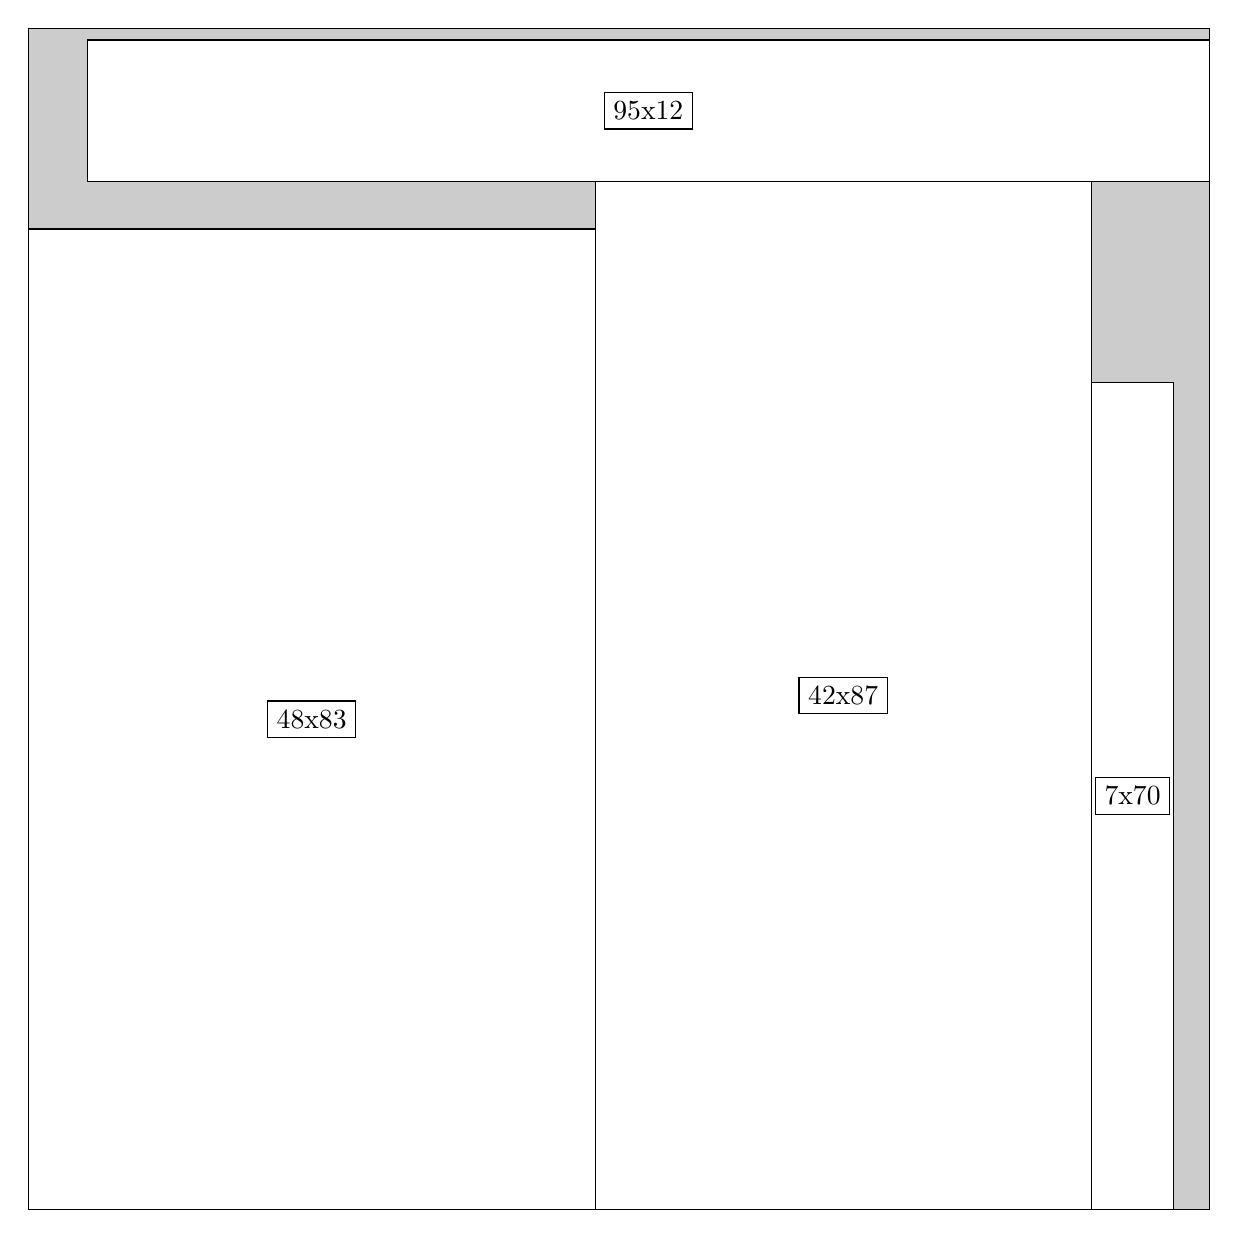
\begin{tikzpicture}[shorten >=1pt,scale=1.0,every node/.style={scale=1.0},->]
\tikzstyle{vertex}=[circle,fill=black!25,minimum size=14pt,inner sep=0pt]
\filldraw[fill=gray!40!white, draw=black] (0,0) rectangle (15.0,15.0);
\foreach \name/\x/\y/\w/\h in {48x83/0.0/0.0/7.199999999999999/12.45,42x87/7.199999999999999/0.0/6.3/13.049999999999999,95x12/0.75/13.049999999999999/14.25/1.7999999999999998,7x70/13.5/0.0/1.05/10.5}
\filldraw[fill=white!40!white, draw=black] (\x,\y) rectangle node[draw] (\name) {\name} ++(\w,\h);
\end{tikzpicture}


w =48 , h =83 , x =0 , y =0 , v =3984
\par
w =42 , h =87 , x =48 , y =0 , v =3654
\par
w =95 , h =12 , x =5 , y =87 , v =1140
\par
w =7 , h =70 , x =90 , y =0 , v =490
\par
\newpage


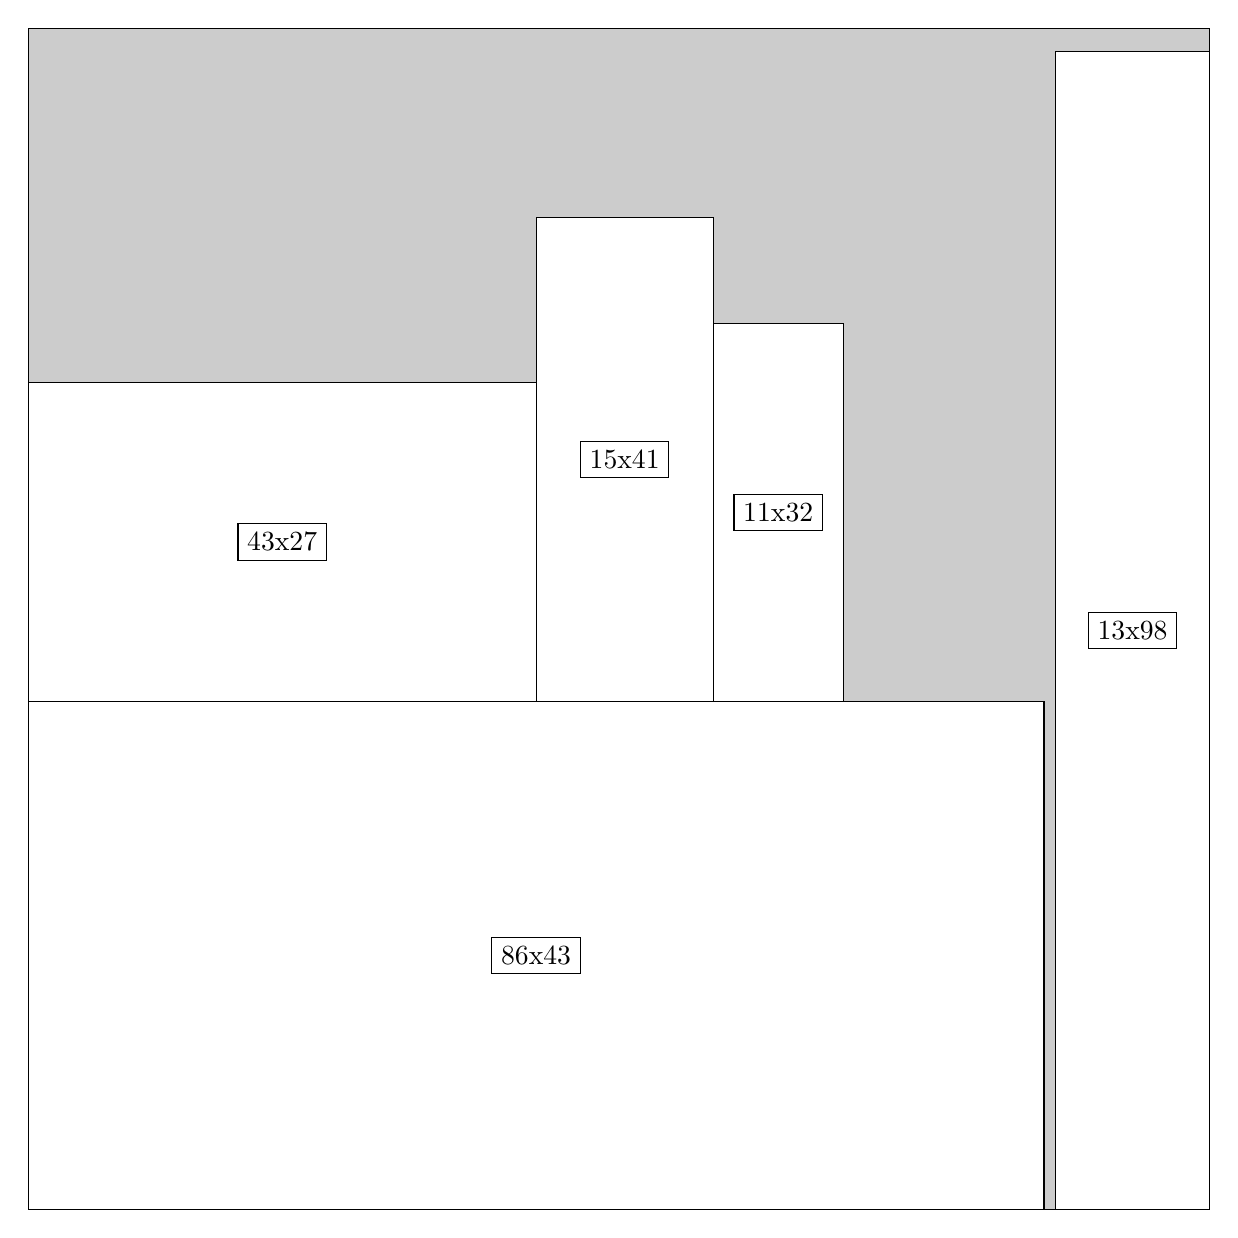
\begin{tikzpicture}[shorten >=1pt,scale=1.0,every node/.style={scale=1.0},->]
\tikzstyle{vertex}=[circle,fill=black!25,minimum size=14pt,inner sep=0pt]
\filldraw[fill=gray!40!white, draw=black] (0,0) rectangle (15.0,15.0);
\foreach \name/\x/\y/\w/\h in {86x43/0.0/0.0/12.9/6.45,13x98/13.049999999999999/0.0/1.95/14.7,43x27/0.0/6.45/6.45/4.05,15x41/6.45/6.45/2.25/6.1499999999999995,11x32/8.7/6.45/1.65/4.8}
\filldraw[fill=white!40!white, draw=black] (\x,\y) rectangle node[draw] (\name) {\name} ++(\w,\h);
\end{tikzpicture}


w =86 , h =43 , x =0 , y =0 , v =3698
\par
w =13 , h =98 , x =87 , y =0 , v =1274
\par
w =43 , h =27 , x =0 , y =43 , v =1161
\par
w =15 , h =41 , x =43 , y =43 , v =615
\par
w =11 , h =32 , x =58 , y =43 , v =352
\par
\newpage


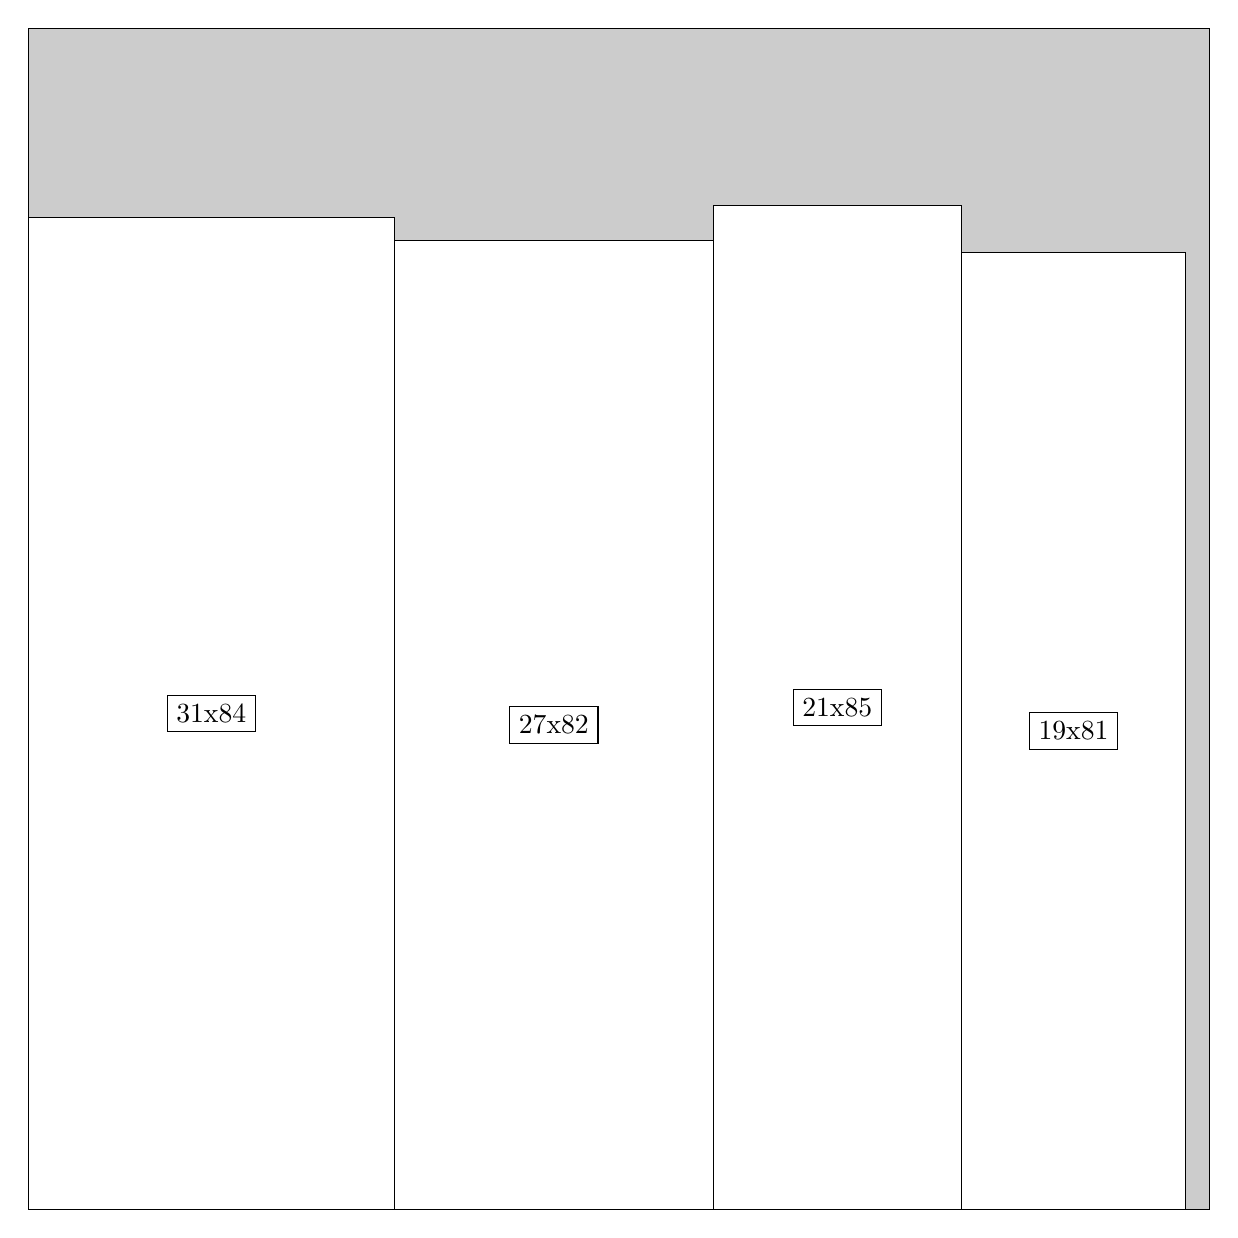
\begin{tikzpicture}[shorten >=1pt,scale=1.0,every node/.style={scale=1.0},->]
\tikzstyle{vertex}=[circle,fill=black!25,minimum size=14pt,inner sep=0pt]
\filldraw[fill=gray!40!white, draw=black] (0,0) rectangle (15.0,15.0);
\foreach \name/\x/\y/\w/\h in {31x84/0.0/0.0/4.6499999999999995/12.6,27x82/4.6499999999999995/0.0/4.05/12.299999999999999,21x85/8.7/0.0/3.15/12.75,19x81/11.85/0.0/2.85/12.15}
\filldraw[fill=white!40!white, draw=black] (\x,\y) rectangle node[draw] (\name) {\name} ++(\w,\h);
\end{tikzpicture}


w =31 , h =84 , x =0 , y =0 , v =2604
\par
w =27 , h =82 , x =31 , y =0 , v =2214
\par
w =21 , h =85 , x =58 , y =0 , v =1785
\par
w =19 , h =81 , x =79 , y =0 , v =1539
\par
\newpage


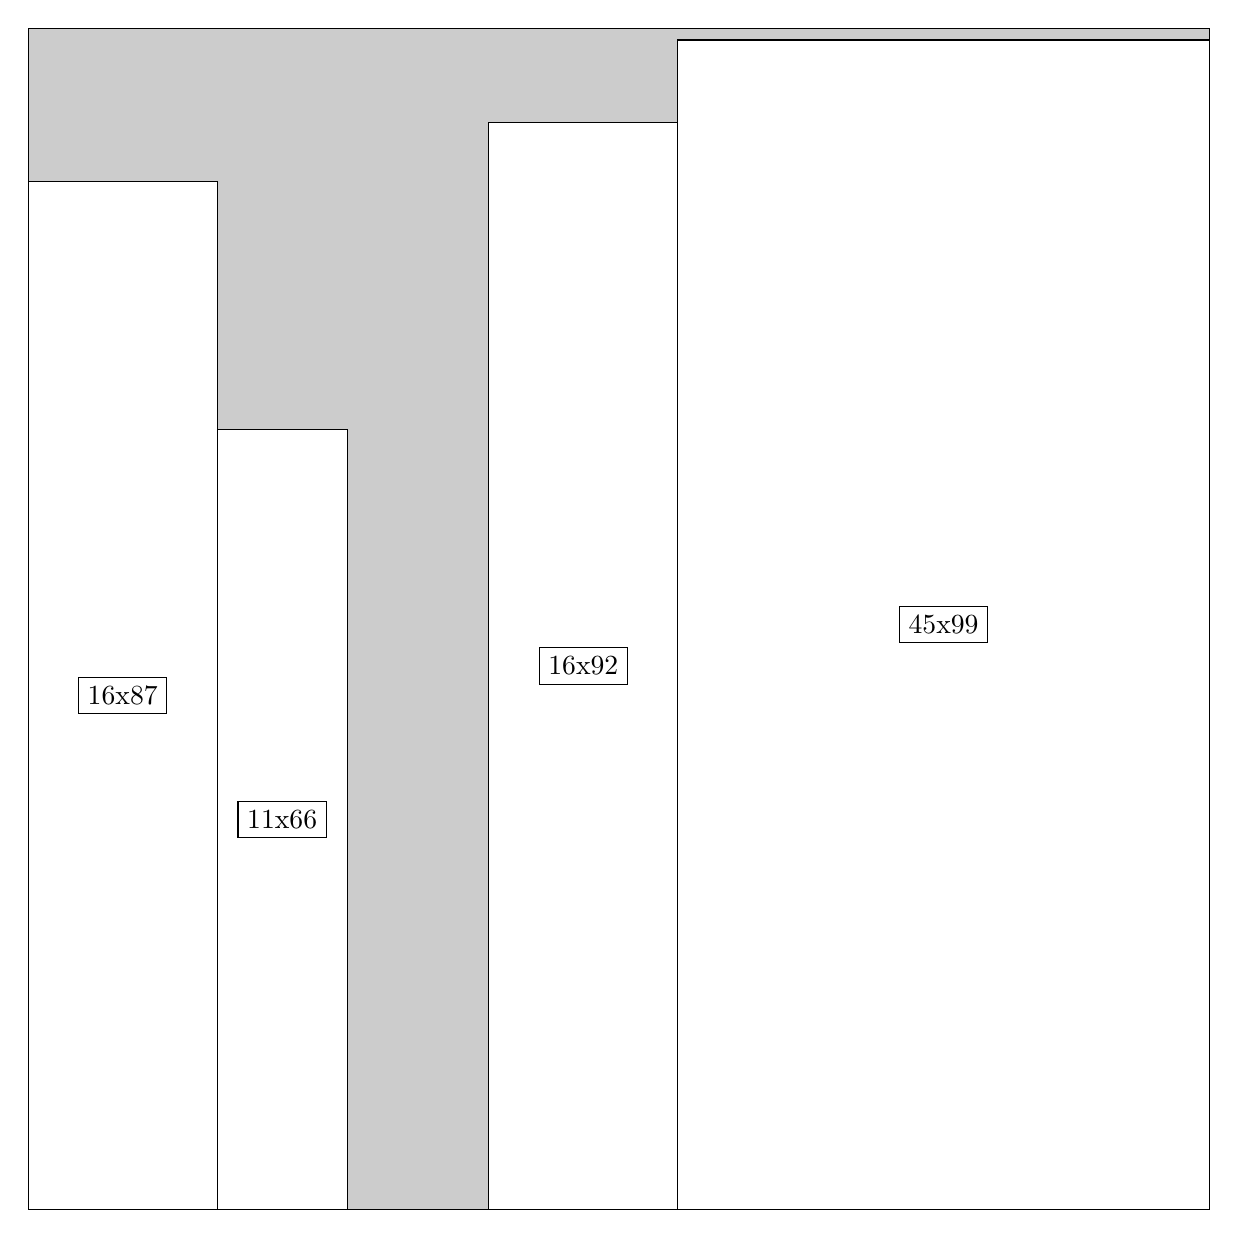
\begin{tikzpicture}[shorten >=1pt,scale=1.0,every node/.style={scale=1.0},->]
\tikzstyle{vertex}=[circle,fill=black!25,minimum size=14pt,inner sep=0pt]
\filldraw[fill=gray!40!white, draw=black] (0,0) rectangle (15.0,15.0);
\foreach \name/\x/\y/\w/\h in {45x99/8.25/0.0/6.75/14.85,16x92/5.85/0.0/2.4/13.799999999999999,16x87/0.0/0.0/2.4/13.049999999999999,11x66/2.4/0.0/1.65/9.9}
\filldraw[fill=white!40!white, draw=black] (\x,\y) rectangle node[draw] (\name) {\name} ++(\w,\h);
\end{tikzpicture}


w =45 , h =99 , x =55 , y =0 , v =4455
\par
w =16 , h =92 , x =39 , y =0 , v =1472
\par
w =16 , h =87 , x =0 , y =0 , v =1392
\par
w =11 , h =66 , x =16 , y =0 , v =726
\par
\newpage


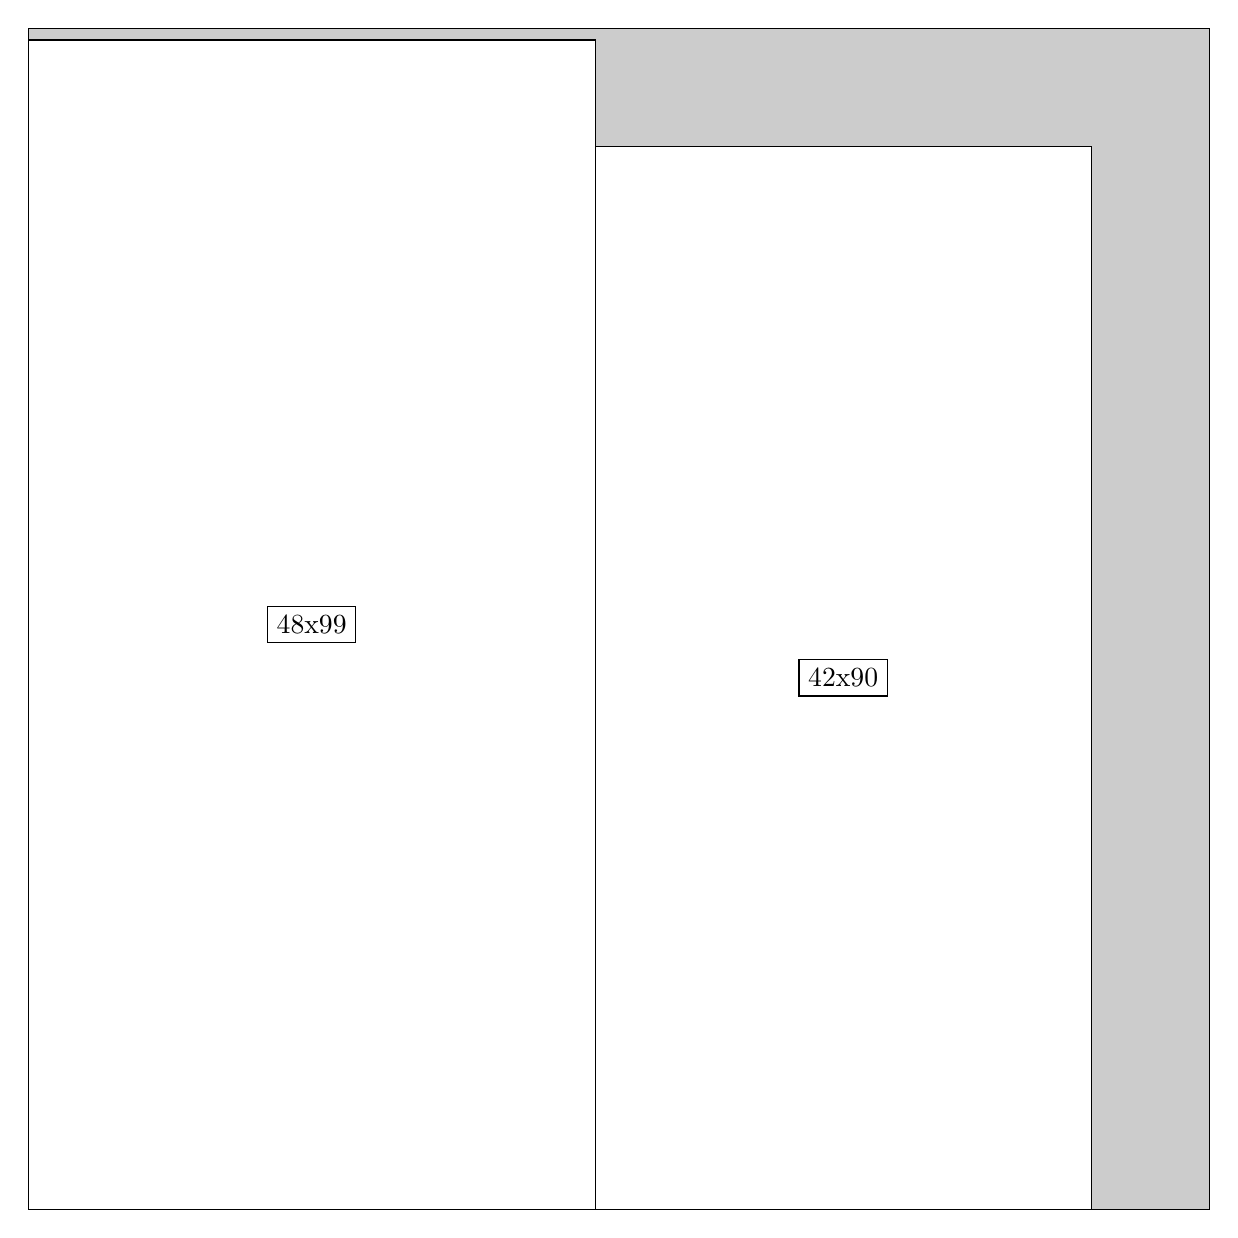
\begin{tikzpicture}[shorten >=1pt,scale=1.0,every node/.style={scale=1.0},->]
\tikzstyle{vertex}=[circle,fill=black!25,minimum size=14pt,inner sep=0pt]
\filldraw[fill=gray!40!white, draw=black] (0,0) rectangle (15.0,15.0);
\foreach \name/\x/\y/\w/\h in {42x90/7.199999999999999/0.0/6.3/13.5,48x99/0.0/0.0/7.199999999999999/14.85}
\filldraw[fill=white!40!white, draw=black] (\x,\y) rectangle node[draw] (\name) {\name} ++(\w,\h);
\end{tikzpicture}


w =42 , h =90 , x =48 , y =0 , v =3780
\par
w =48 , h =99 , x =0 , y =0 , v =4752
\par
\newpage


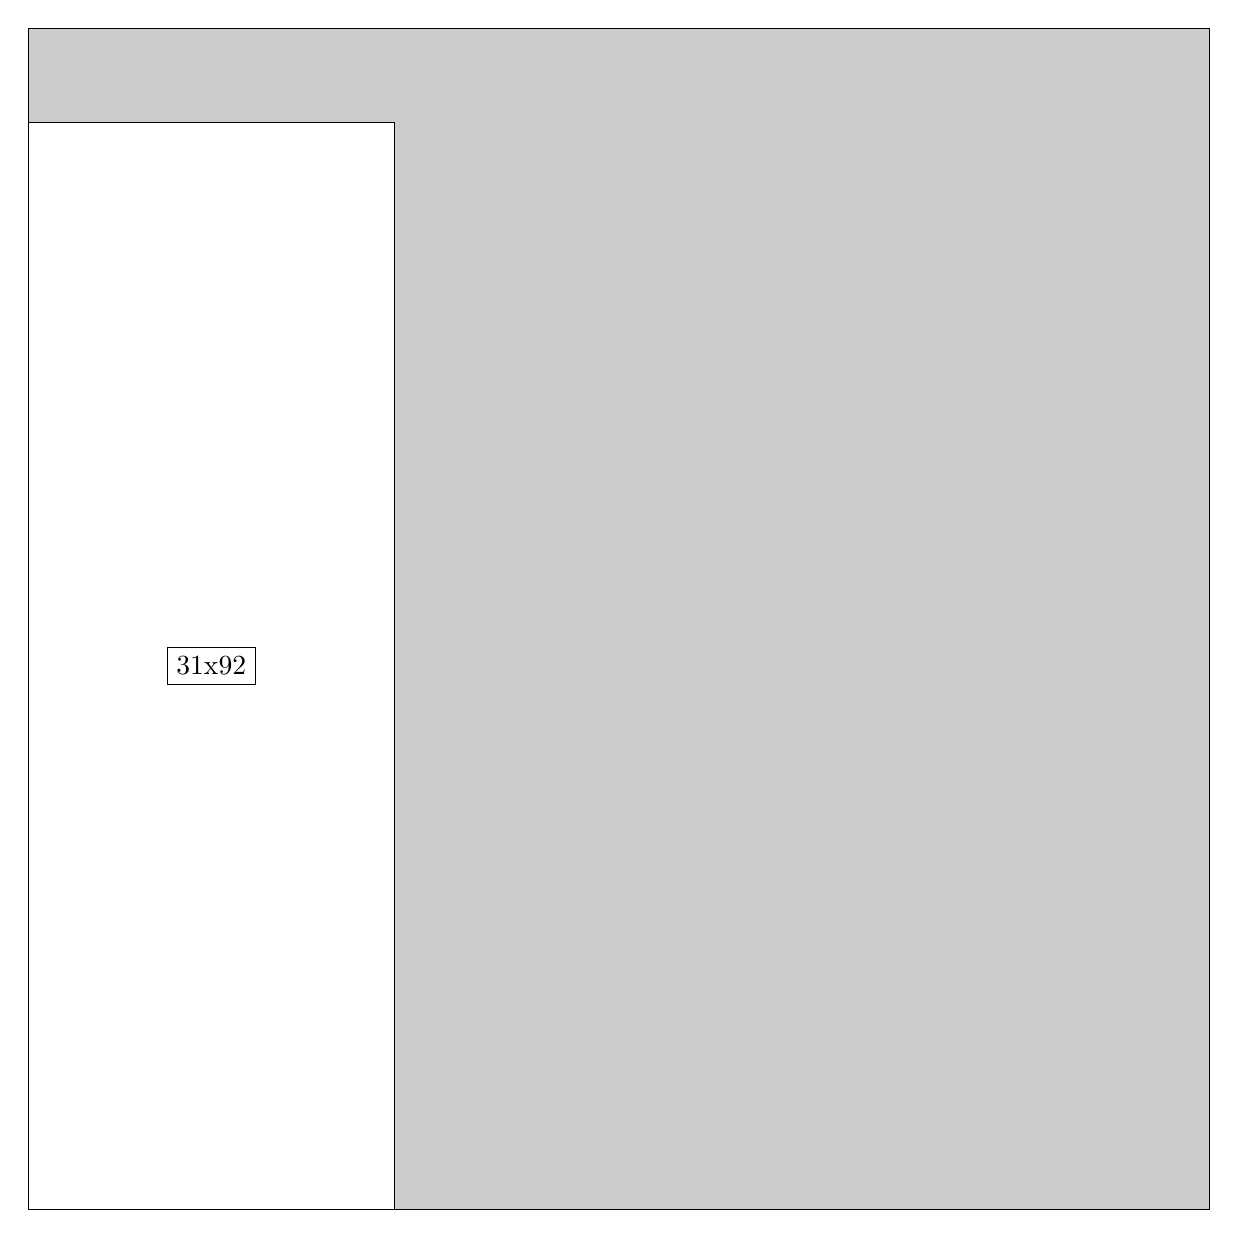
\begin{tikzpicture}[shorten >=1pt,scale=1.0,every node/.style={scale=1.0},->]
\tikzstyle{vertex}=[circle,fill=black!25,minimum size=14pt,inner sep=0pt]
\filldraw[fill=gray!40!white, draw=black] (0,0) rectangle (15.0,15.0);
\foreach \name/\x/\y/\w/\h in {31x92/0.0/0.0/4.6499999999999995/13.799999999999999}
\filldraw[fill=white!40!white, draw=black] (\x,\y) rectangle node[draw] (\name) {\name} ++(\w,\h);
\end{tikzpicture}


w =31 , h =92 , x =0 , y =0 , v =2852
\par
\newpage


\end{document}